% A LaTeX template for EXECUTIVE SUMMARY of the MSc Thesis submissions to 
% Politecnico di Milano (PoliMi) - School of Industrial and Information Engineering
%
% P. F. Antonietti, S. Bonetti, A. Gruttadauria, G. Mescolini, A. Zingaro
% e-mail: template-tesi-ingind@polimi.it
%
% Last Revision: October 2021
%
% Copyright 2021 Politecnico di Milano, Italy. Inc. All rights reserved.

\documentclass[11pt,a4paper,twocolumn]{article}

%------------------------------------------------------------------------------
%	REQUIRED PACKAGES AND  CONFIGURATIONS
%------------------------------------------------------------------------------
% PACKAGES FOR TITLES
\usepackage{titlesec}
\usepackage{color}

% PACKAGES FOR LANGUAGE AND FONT
\usepackage[utf8]{inputenc}
\usepackage[english]{babel}
\usepackage[T1]{fontenc} % Font encoding

% PACKAGES FOR IMAGES
\usepackage{graphicx}
\graphicspath{{Images/}} % Path for images' folder
\usepackage{eso-pic} % For the background picture on the title page
\usepackage{subfig} % Numbered and caption subfigures using \subfloat
\usepackage{caption} % Coloured captions
\usepackage{transparent}

% STANDARD MATH PACKAGES
\usepackage{amsmath}
\usepackage{amsthm}
\usepackage{bm}
\usepackage[overload]{empheq}  % For braced-style systems of equations

% PACKAGES FOR TABLES
\usepackage{tabularx}
\usepackage{longtable} % tables that can span several pages
\usepackage{colortbl}

% PACKAGES FOR ALGORITHMS (PSEUDO-CODE)
\usepackage{algorithm}
\usepackage{algorithmic}

% PACKAGES FOR REFERENCES & BIBLIOGRAPHY
\usepackage[colorlinks=true,linkcolor=black,anchorcolor=black,citecolor=black,filecolor=black,menucolor=black,runcolor=black,urlcolor=black]{hyperref} % Adds clickable links at references
\usepackage{cleveref}
\usepackage[square, numbers, sort&compress]{natbib} % Square brackets, citing references with numbers, citations sorted by appearance in the text and compressed
\bibliographystyle{plain} % You may use a different style adapted to your field

% PACKAGES FOR THE APPENDIX
\usepackage{appendix}

% PACKAGES FOR ITEMIZE & ENUMERATES 
\usepackage{enumitem}

% OTHER PACKAGES
\usepackage{amsthm,thmtools,xcolor} % Coloured "Theorem"
\usepackage{comment} % Comment part of code
\usepackage{fancyhdr} % Fancy headers and footers
\usepackage{lipsum} % Insert dummy text
\usepackage{tcolorbox} % Create coloured boxes (e.g. the one for the key-words)
\usepackage{stfloats} % Correct position of the tables

%-------------------------------------------------------------------------
%	NEW COMMANDS DEFINED
%-------------------------------------------------------------------------
% EXAMPLES OF NEW COMMANDS -> here you see how to define new commands
\newcommand{\bea}{\begin{eqnarray}} % Shortcut for equation arrays
\newcommand{\eea}{\end{eqnarray}}
\newcommand{\e}[1]{\times 10^{#1}}  % Powers of 10 notation
\newcommand{\mathbbm}[1]{\text{\usefont{U}{bbm}{m}{n}#1}} % From mathbbm.sty
\newcommand{\pdev}[2]{\frac{\partial#1}{\partial#2}}
% NB: you can also override some existing commands with the keyword \renewcommand

%----------------------------------------------------------------------------
%	ADD YOUR PACKAGES (be careful of package interaction)
%----------------------------------------------------------------------------


%----------------------------------------------------------------------------
%	ADD YOUR DEFINITIONS AND COMMANDS (be careful of existing commands)
%----------------------------------------------------------------------------


% Do not change Configuration_files/config.tex file unless you really know what you are doing. 
% This file ends the configuration procedures (e.g. customizing commands, definition of new commands)
% Set the geometric layout of the document
\usepackage{geometry}
\geometry{
  top=3cm,
  left = 2.0cm,
  right = 2.0cm,
  bottom=2cm,
  headheight= 2cm,
  headsep= 0cm,
}
\raggedbottom

% Create color bluePoli (-> manuale grafica coordinata:  https://www.polimi.it/fileadmin/user_upload/il_Politecnico/grafica-coordinata/2015_05_11_46xy_manuale_grafica_coordinata.pdf)
\definecolor{bluePoli}{cmyk}{0.4,0.1,0,0.4}

% Custom theorem environments
\declaretheoremstyle[
  shaded={rulecolor=bluePoli!20, rulewidth=1pt, bgcolor=bluePoli!5},
  headfont=\color{bluePoli}\normalfont\bfseries,
  bodyfont=\color{black}\normalfont,
]{colored}

\captionsetup[figure]{labelfont={color=bluePoli}} % Set colour of the captions
\captionsetup[table]{labelfont={color=bluePoli}} % Set colour of the captions
\captionsetup[algorithm]{labelfont={color=bluePoli}} % Set colour of the captions

\theoremstyle{colored}
\newtheorem{theorem}{Theorem}[section]
\newtheorem{proposition}{Proposition}[section]
\newtheorem{definition}{Definition}[section]
\newtheorem*{remark}{Remark}
\newtheorem{lemma}{Lemma}[section]

% Enhances the features of the standard "table" and "tabular" environments.
\newcommand\T{\rule{0pt}{2.6ex}}
\newcommand\B{\rule[-1.2ex]{0pt}{0pt}}

% Algorithm description
\newcounter{algsubstate}
\renewcommand{\thealgsubstate}{\alph{algsubstate}}
\newenvironment{algsubstates}{
    \setcounter{algsubstate}{0}%
    \renewcommand{\STATE}{%
    \stepcounter{algsubstate}%
    \Statex {\small\thealgsubstate:}\space}
    }{}

% Custom theorem environment
\newcolumntype{L}[1]{>{\raggedright\let\newline\\\arraybackslash\hspace{0pt}}m{#1}}
\newcolumntype{C}[1]{>{\centering\let\newline\\\arraybackslash\hspace{0pt}}m{#1}}
\newcolumntype{R}[1]{>{\raggedleft\let\newline\\\arraybackslash\hspace{0pt}}m{#1}}

% Custom itemize environment
\setlist[itemize,1]{label=$\bullet$}
\setlist[itemize,2]{label=$\circ$}
\setlist[itemize,3]{label=$-$}
\setlist{nosep}

% Set separation of columns
\setlength{\columnsep}{30pt}

% Create command for background pic
\newcommand\BackgroundPic{% Adding background picture
	\put(230,358){
		\parbox[b][\paperheight]{\paperwidth}{%
			\vfill
			\centering
			\transparent{0.2}
			
\includegraphics[width=0.8\paperwidth]{raggiera_polimi.eps}%
			\vfill
}}}

% Set indentation
%\setlength\parindent{0pt}

% Custom title commands
\titleformat{\section}
{\color{bluePoli}\normalfont\Large\bfseries}
{\color{bluePoli}\thesection.}{1em}{}
\titlespacing*{\section}
{0pt}{2ex}{1ex}

\titleformat{\subsection}
{\color{bluePoli}\normalfont\large\bfseries}
{\color{bluePoli}\thesubsection.}{1em}{}
\titlespacing*{\subsection}
{0pt}{2ex}{1ex}

\titleformat{\subsubsection}
{\color{bluePoli}\normalfont\normalsize\bfseries}
{\color{bluePoli}\thesubsubsection.}{1em}{}
\titlespacing*{\subsubsection}
{0pt}{2ex}{1ex}

% Custom headers and footers
\pagestyle{fancy}
\fancyhf{}

\fancyfoot{}
\fancyfoot[C]{\thepage} % page
\renewcommand{\headrulewidth}{0mm} % headrule width
\renewcommand{\footrulewidth}{0mm} % footrule width

\makeatletter
\patchcmd{\headrule}{\hrule}{\color{black}\hrule}{}{} % headrule
\patchcmd{\footrule}{\hrule}{\color{black}\hrule}{}{} % footrule
\makeatother

% -> Create the header
\chead[C]{
\centering
\begin{tcolorbox}[arc=0pt, boxrule=0pt, colback=bluePoli!60, width=\textwidth, colupper=white]
    
\includegraphics[width=0.2\textwidth]{mimesis.png}
\end{tcolorbox}
}


% Insert here the info that will be displayed into your Title page 
% -> title of your work
\renewcommand{\title}{A Modified Neural Modes Approach for Soft Tissue Simulation}
% -> author name and surname
\renewcommand{\author}{Name Surname}
% -> MSc course
\newcommand{\course}{Mathematical Engineering - Ingegneria Matematica}
% -> advisor name and surname
\newcommand{\advisor}{Prof. Stefano Pagani}
% IF AND ONLY IF you need to modify the co-supervisors you also have to modify the file Configuration_files/title_page.tex (ONLY where it is marked)
\newcommand{\firstcoadvisor}{Dr. Stéphane Cotin} % insert if any otherwise comment
%\newcommand{\secondcoadvisor}{Name Surname} % insert if any otherwise comment
% -> academic year
\newcommand{\YEAR}{2024-2025}

%-------------------------------------------------------------------------
%	BEGIN OF YOUR DOCUMENT
%-------------------------------------------------------------------------
\begin{document}

%-----------------------------------------------------------------------------
% TITLE PAGE
%-----------------------------------------------------------------------------
% Do not change Configuration_files/TitlePage.tex (Modify it IF AND ONLY IF you need to add or delete the Co-advisors)
% This file creates the Title Page of the document
% DO NOT REMOVE SPACES BETWEEN LINES!

%\twocolumn[{\begin{@twocolumnfalse}

\AddToShipoutPicture*{\BackgroundPic}

\hspace{-0.6cm}
\includegraphics[width=0.6\textwidth]{logo_polimi_ing_indinf.eps}

\vspace{-1mm}
\fontsize{0.3cm}{0.5cm}\selectfont \bfseries \textsc{\color{bluePoli} Report}\\

\vspace{-0.2cm}
\Large{\textbf{\color{bluePoli}{\title}}}\\

\vspace{-0.2cm}
\fontsize{0.3cm}{0.5cm}\selectfont \bfseries \textsc{\color{bluePoli} \course}\\

\vspace{-0.2cm}
\fontsize{0.3cm}{0.5cm} \selectfont \bfseries Authors: \textsc{\textbf{\author}}\\

%\vspace{-0.4cm}
%\fontsize{0.3cm}{0.5cm}\selectfont \bfseries Advisor: \textsc{\textbf{\advisor}}\\

% if only ONE co-advisor is present:
%\vspace{-0.4cm}
%\fontsize{0.3cm}{0.5cm}\selectfont \bfseries Co-advisor: \textsc{\textbf{\firstcoadvisor}}\\
% if more than one co-advisors are present:
%\vspace{-0.4cm}
%\fontsize{0.3cm}{0.5cm}\selectfont \bfseries Co-advisors: \textsc{\textbf{\firstcoadvisor}}\textsc{\textbf{\secondcoadvisor}}\\

\vspace{-0.4cm}
\fontsize{0.3cm}{0.5cm}\selectfont \bfseries Academic year: \textsc{\textbf{\YEAR}}

\small \normalfont

\vspace{11pt}

\centerline{\rule{1.0\textwidth}{0.4pt}}

%\vspace{15pt}
%\end{@twocolumnfalse}}]

\thispagestyle{plain} % In order to not show the header in the first page


%%%%%%%%%%%%%%%%%%%%%%%%%%%%%%
%%     THESIS MAIN TEXT     %%
%%%%%%%%%%%%%%%%%%%%%%%%%%%%%%

%-----------------------------------------------------------------------------
% INTRODUCTION
%-----------------------------------------------------------------------------

\section{Introduction}
\label{sec:es:introduction}

Accurate simulation of object deformation is crucial across many scientific and engineering disciplines, particularly in fields like biomedical engineering for applications such as surgical simulation. Traditional Finite Element Methods (FEM) provide high accuracy but are computationally demanding, making real-time applications challenging, especially when dealing with large, nonlinear deformations characteristic of soft tissues. Reduced-order models (ROMs) offer a way to accelerate simulations by reducing the problem's dimensionality, but standard linear ROMs struggle to capture the complex, nonlinear behavior accurately. This executive summary outlines a thesis that investigates and enhances the "Neural Modes" framework, a hybrid approach that combines the efficiency of linear modal analysis with the power of deep learning to enable accurate and computationally tractable simulations of nonlinear soft tissue deformation. The work builds upon existing research, proposing modifications to improve the framework's performance and applicability.

\section{Mathematical Framework}
\label{sec:es:mathematical_framework}

Simulating the deformation of soft tissues requires a mathematical framework capable of describing their nonlinear mechanical behavior. We model the material using the hyperelastic Neo-Hookean constitutive law, which is suitable for large deformations. The behavior of the material is governed by its strain-energy density function $\Psi$, which for the Neo-Hookean model is given by:
\begin{equation}
    \Psi(\bm{F}) = \frac{\mu}{2} (\text{tr}(\bm{C}) - 3 - 2\ln(J)) + \frac{\lambda}{4} (J^2 - 1 - 2\ln(J)),
\label{eq:es:neo_hookean_energy}
\end{equation}
where $\bm{F}$ is the deformation gradient, $\bm{C} = \bm{F}^T \bm{F}$ is the right Cauchy-Green tensor, $J = \det(\bm{F})$, and $\mu$ and $\lambda$ are Lamé parameters related to the material's Young's modulus and Poisson's ratio \cite{Ogden_1997}. The first Piola-Kirchhoff stress tensor $\bm{P}$, which relates forces in the reference configuration to areas in the reference configuration, is derived from the strain-energy density function as:
\begin{equation}
    \bm{P} = \frac{\partial \Psi}{\partial \bm{F}}.
\label{eq:es:first_piola_kirchhoff}
\end{equation}
The equations of motion for a deformable body are then expressed in the reference configuration as:
\begin{equation}
    \rho_0 \ddot{\bm{u}} = \nabla_0 \cdot \bm{P} + \bm{B}_0,
\label{eq:es:equations_of_motion}
\end{equation}
where $\rho_0$ is the mass density in the reference configuration, $\ddot{\bm{u}}$ is the acceleration, $\nabla_0 \cdot$ is the divergence operator with respect to the reference configuration, and $\bm{B}_0$ represents body forces per unit volume in the reference configuration.

To reduce the computational cost of solving these nonlinear dynamic equations, we utilize linear modal analysis \cite{Pentland_Williams_1989}. This technique linearizes the system around the undeformed state and solves a generalized eigenvalue problem to find the dominant vibration modes:
\begin{equation}
    \bm{K} \bm{\phi}_i = \omega_i^2 \bm{M} \bm{\phi}_i,
\label{eq:es:eigenvalue_problem}
\end{equation}
where $\bm{K}$ is the linear stiffness matrix, $\bm{M}$ is the mass matrix, $\omega_i^2$ are the squared natural frequencies, and $\bm{\phi}_i$ are the mode shapes. The displacement field is then approximated as a linear combination of the first $m$ modes:
\begin{equation}
    \bm{u}(\bm{X},t) \approx \sum_{i=1}^{m} q_i(t) \bm{\phi}_i(\bm{X}),
\label{eq:es:modal_decomposition}
\end{equation}
where $q_i(t)$ are the time-dependent modal coordinates. Substituting this approximation into the equations of motion and projecting onto the modal basis yields a reduced system of ordinary differential equations for the modal coordinates. The forces acting on the system are also projected onto the modal basis, resulting in modal forces $\bm{f}_{modal}$:
\begin{equation}
    \bm{f}_{modal} = \bm{\Phi}^T \bm{f}_{external},
\label{eq:es:modal_forces}
\end{equation}
where $\bm{\Phi}$ is the matrix whose columns are the mode shapes $\bm{\phi}_i$, and $\bm{f}_{external}$ represents the external forces. While efficient, this linear approximation is only accurate for small deformations.

\section{Enhanced Neural Modes Method}
\label{sec:es:enhanced_neural_modes}

The "Neural Modes" framework, originally proposed by Wang et al. \cite{Wang_Du_Coros_Thomaszewski_2024}, extends linear modal analysis by using a neural network to learn nonlinear corrections to the linear modal displacement. Our work builds upon this foundation, addressing limitations identified in the original self-supervised training approach, particularly its effectiveness for large deformations and sampling of the latent space.

We propose an enhanced Neural Modes framework that employs a supervised learning strategy. A deep residual neural network is trained to predict a nonlinear correction vector $\bm{y}$ based on the linear modal coordinates $\bm{z}$. The total displacement is then the sum of the linear modal displacement $\bm{l} = \bm{\Phi} \bm{z}$ and the learned correction:
\begin{equation}
    \bm{u} = \bm{l} + \bm{y}(\bm{z}).
\label{eq:es:total_displacement}
\end{equation}
The network is trained on a dataset of $(\bm{z}, \bm{u}_{ground\_truth}, E_{ground\_truth})$ pairs generated from full-order nonlinear FEM simulations.

The training utilizes a physics-informed loss function that combines:
\begin{itemize}
    \item An energy loss term comparing the predicted internal energy (derived from the predicted displacement $\bm{u}$) to the ground truth energy.
    \item A displacement loss term comparing the predicted displacement $\bm{u}$ to the ground truth displacement $\bm{u}_{ground\_truth}$.
    \item Additional terms to encourage orthogonality between the linear and nonlinear components and enforce boundary conditions.
\end{itemize}
This supervised, physics-informed approach allows the network to learn accurate nonlinear corrections and generalize well, even with a relatively small amount of training data.

\section{Dynamic Simulation}
\label{sec:es:dynamic_simulation}

For dynamic simulations, the enhanced Neural Modes framework determines the modal coordinates at each time step by solving an optimization problem. This optimization minimizes a cost function that includes terms related to inertia and the internal energy of the configuration predicted by the neural network. While this approach enables dynamic simulation, it relies on an iterative solver (like L-BFGS-B) and does not explicitly incorporate external forces into the optimization in a straightforward manner, which can affect long-term accuracy and stability compared to a fully reduced dynamic system.

\section{Numerical Results}
\label{sec:es:numerical_results}

We validated the enhanced Neural Modes framework on 3D benchmark problems: a cantilever beam and the Stanford bunny, both modeled as Neo-Hookean materials.

Initial analysis determined the optimal number of linear modes required for a sufficient basis. As illustrated in figures showing the cantilever beam's deformation under increasing load (e.g., Figure \ref{fig:static_rmse_distribution}), the linear modal approximation deviates significantly from the ground truth at larger displacements. Figure \ref{fig:optimal_number_modes} shows the RMSE of the displacement field as a function of the number of modes used, indicating that the error stabilizes around 20 modes, with 7 modes being sufficient for our use case.

\begin{figure}[H]
    \centering
    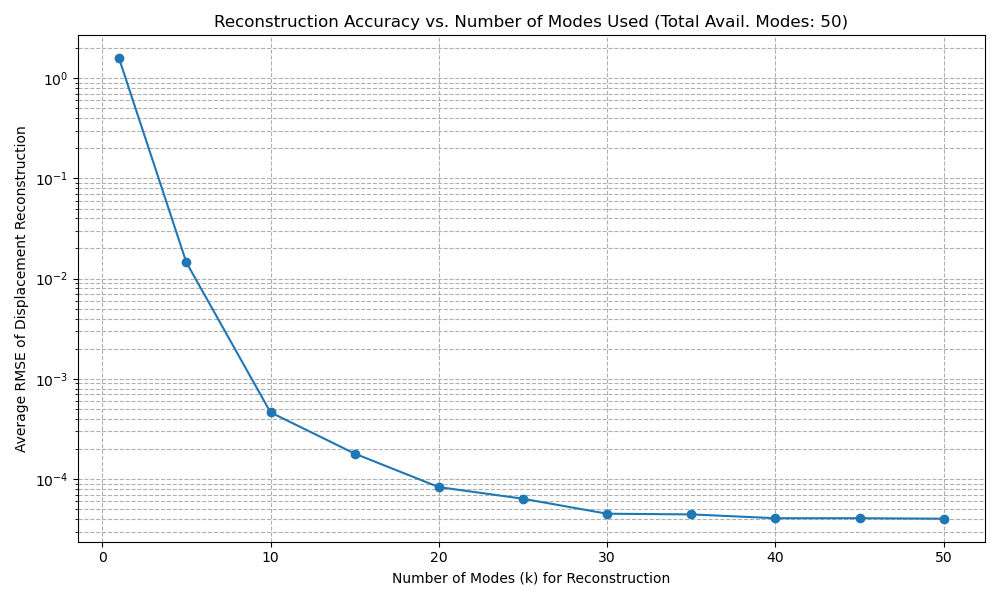
\includegraphics[width=0.3\textwidth]{Images/rmse_vs_modes.png}
    \caption{RMSE of the displacement field as a function of the number of modes used.}
    \label{fig:optimal_number_modes}
\end{figure}

Comparison between a self-supervised training approach (similar to the original work \cite{Wang_Du_Coros_Thomaszewski_2024}) and our supervised method showed that the supervised training significantly improved the model's ability to capture large deformations, outperforming the self-supervised model which performed at best comparably to linear modes (see Figure \ref{fig:self_supervised_validation_mse_comparison} for error comparisons).

\begin{figure}[H]
    \centering
    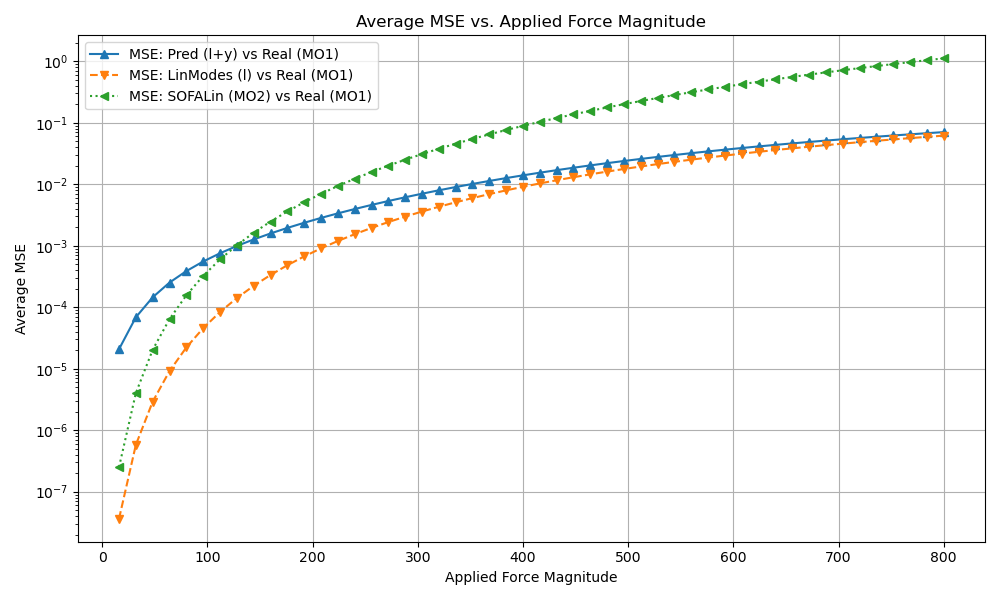
\includegraphics[width=0.3\textwidth]{Images/self_supervised_mse.png}
    \caption{Average MSE between 40 different simulations with randomly applied forces. The neural modes model (blue) is compared against the linear modes model (orange) and the linear FEM model (green), all evaluated against the nonlinear FEM ground truth. The self-supervised model performs at most as well as the linear modes, as shown by the MSE values.}
    \label{fig:self_supervised_validation_mse_comparison}
\end{figure}

Static validation on unseen configurations demonstrated that the supervised Neural Modes model accurately predicted displacement fields, significantly outperforming linear modes and linear FEM, especially in the nonlinear deformation regime. Figure \ref{fig:static_mse_comparison} presents the average MSE comparison for the cantilever beam, showing the superior performance of neural modes in the nonlinear range. Figure \ref{fig:static_rmse_distribution} provides a visual comparison of the predicted deformation patterns for the cantilever beam, highlighting how the neural modes capture the pronounced bending curvature missed by linear methods.

\begin{figure}[H]
    \centering
    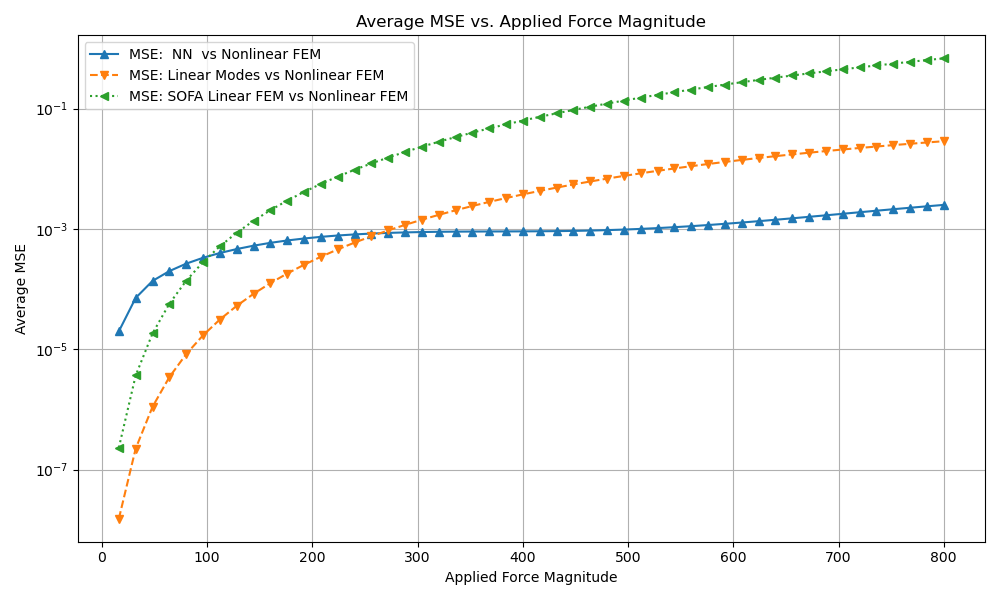
\includegraphics[width=0.3\textwidth]{Images/beam_static_mse.png}
    \caption{Average MSE between 40 different simulations with randomly applied forces. The neural modes model (blue) is compared against the linear modes model (orange) and the linear FEM model (green), all evaluated against the nonlinear FEM ground truth. The neural modes model significantly outperforms the linear modes, especially in the nonlinear regime.}
    \label{fig:static_mse_comparison}
\end{figure}

\begin{figure}[H]
    \centering
    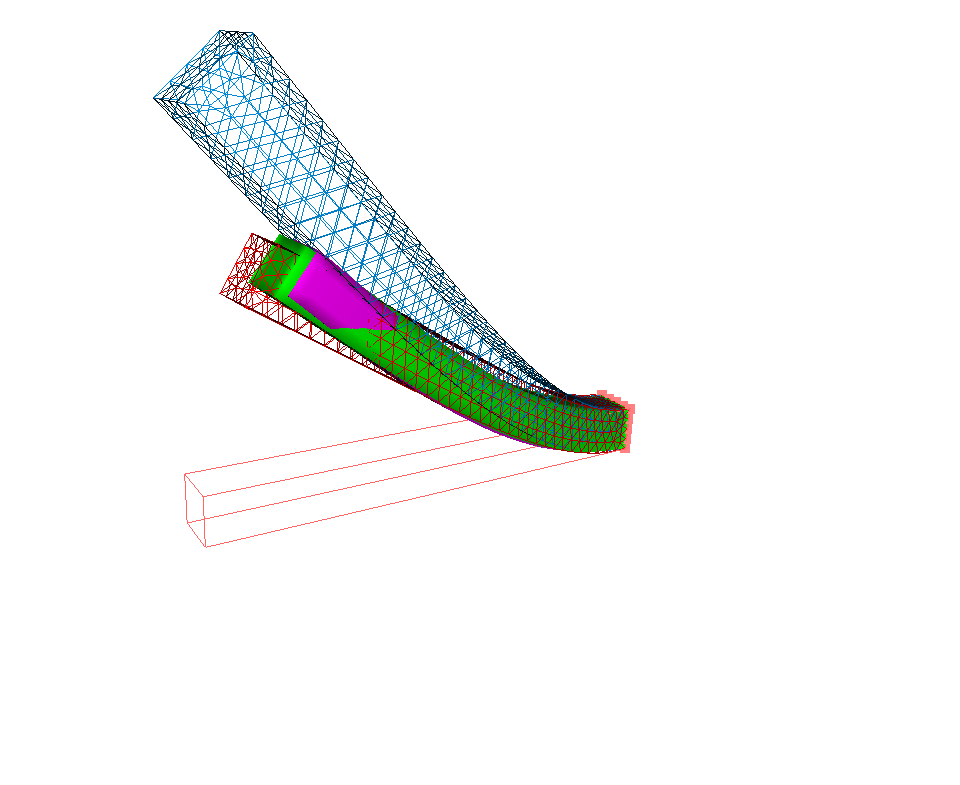
\includegraphics[width=0.3\textwidth]{Images/sofa_example_beam.png}
    \caption{Example of a static reconstruction in the case of the beam. The magenta beam represents the neural network prediction, the green one is the ground truth, the red wireframe represents the linear modes and the blue wireframe is the linear FEM model.}
    \label{fig:static_rmse_distribution}
\end{figure}

The model also predicted internal energy much closer to the ground truth, indicating better physical consistency (Figure \ref{fig:static_energy_beam} shows energy error plots for the cantilever beam).

\begin{figure}[H]
    \centering
    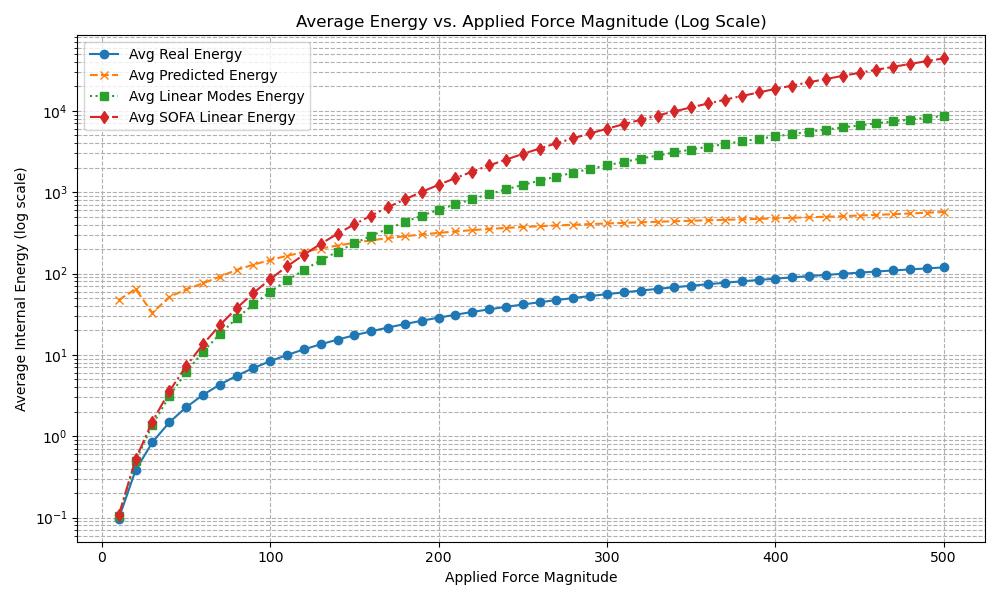
\includegraphics[width=0.3\textwidth]{Images/beam_static_energy.png}
    \caption{Internal mechanical energy of the beam as a function of the applied force. The orange line represents the energy computed by the neural network model, while the blue line is the ground truth obtained from the nonlinear FEM solution. The red line represents the energy computed by the FEM with linear elasticity and the green line is the energy computed by the linear modes model.}
    \label{fig:static_energy_beam}
\end{figure}



Dynamic validation, initialized with full FEM steps, showed that the Neural Modes model maintained internal energy levels much closer to the ground truth over time compared to linear modes, which exhibited significant energy divergence (Figure \ref{fig:dynamic_validation_energy_comparison}). While displacement accuracy still showed room for improvement over extended periods (Figure \ref{fig:dynamic_validation_mse_comparison}), the enhanced framework yielded physically more plausible dynamic predictions, despite being trained only on static data.

\begin{figure}[H]
    \centering
    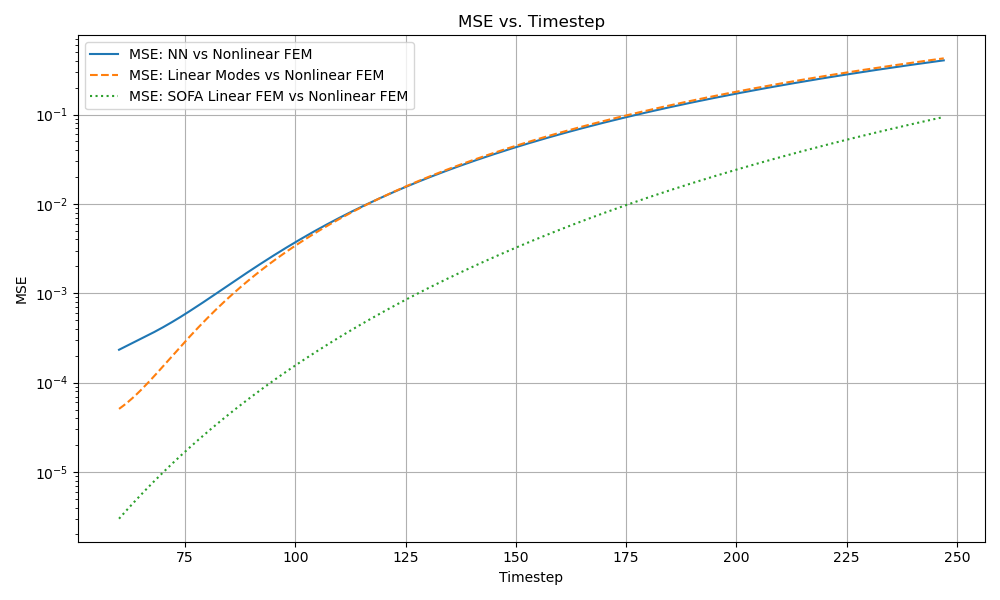
\includegraphics[width=0.3\textwidth]{Images/beam_dynamic_mse.png}
    \caption{MSE of the displacement field as a function of time for the dynamic validation of the cantilever beam. The neural modes model (blue) and the linear modes model (orange) are compared against the ground truth obtained from the nonlinear FEM solution (green). The neural modes model performs slightly better than the linear modes model, especially after the first few time steps.}
    \label{fig:dynamic_validation_mse_comparison}
    \end{figure}

\begin{figure}[htb]
    \centering
    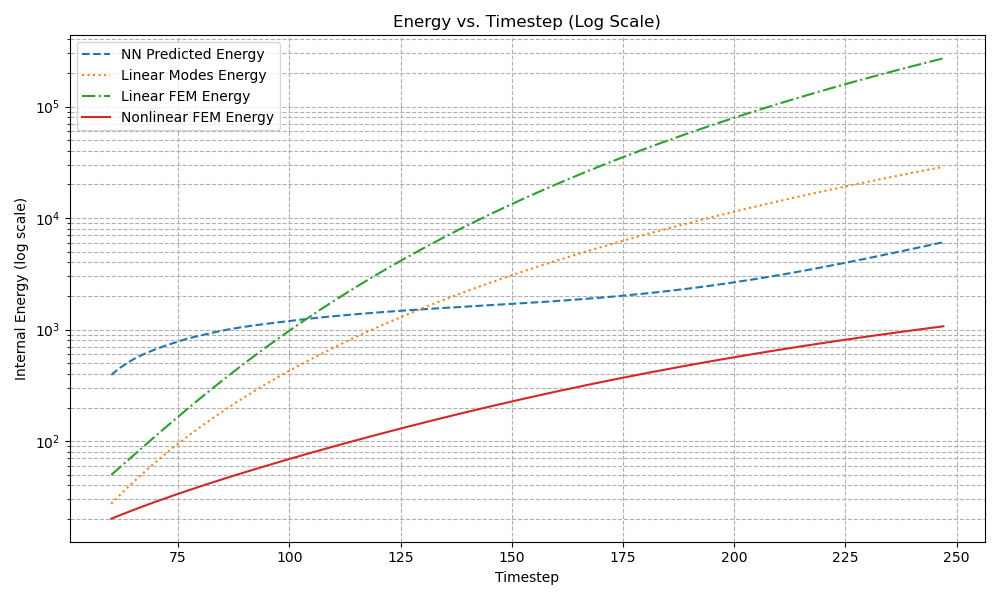
\includegraphics[width=0.3\textwidth]{Images/beam_dynamic_energy.png}
    \caption{Internal mechanical energy of the cantilever beam as a function of time for the dynamic validation. The neural modes model (blue) and the linear modes model (orange) are compared against the ground truth obtained from the nonlinear FEM solution (green). The neural modes model manages to keep the energy at a level that is much closer to the ground truth, while the linear modes model diverges significantly from it.}
    \label{fig:dynamic_validation_energy_comparison}
    \end{figure}

\section{Conclusion and Future Work}
\label{sec:es:conclusion}

This thesis successfully enhanced the Neural Modes framework through a supervised learning strategy with a physics-informed loss function. This modification addressed limitations of the original self-supervised approach \cite{Wang_Du_Coros_Thomaszewski_2024}, enabling accurate capture of large, nonlinear soft tissue deformations with reduced data requirements. The numerical results demonstrate significant improvements over traditional linear methods in terms of displacement accuracy and energy conservation in the nonlinear regime, while maintaining computational efficiency suitable for real-time applications.

Future work should focus on improving dynamic simulation accuracy, potentially by exploring more sophisticated temporal integration schemes or incorporating a fully reduced dynamic model. Extending the framework to handle more complex external forces and different material models (e.g., viscoelasticity) would broaden its applicability. Exploring alternative neural network architectures could also yield further improvements in accuracy or efficiency. The enhanced Neural Modes framework represents a promising step towards efficient, accurate, and physically consistent simulation of nonlinear mechanics, with significant potential for applications in biomedical engineering and beyond.


%---------------------------------------------------------------------------
%  BIBLIOGRAPHY
%---------------------------------------------------------------------------
% Remember to insert here only the essential bibliography of your work
\bibliography{bibliography.bib} % automatically inserted and ordered with this command 

\end{document}